\section{Analysis}
\label{sec:analysis}
We start the project by analyzing the basic requirements for a truck platooning system. There are several factors one should consider, such as a reliable communication system to ensure smooth coordination among the vehicles in the platooning system, the ability to maintain a consistent speed and a minimum distance between vehicles to ensure safe operation, efficient fuel consumption, and the ability to adapt to changes in traffic conditions. It is important to develop a system that can accurately detect and respond to the movements of the leader and follower trucks in real-time and should be able to respond to emergencies \cite{b2}.\\
Thus, based on this, we can develop a use case for a truck platooning system that enhances safety and efficiency in long-haul transportation. As depicted in Figure \ref{img:usecase}, we establish two main actors that can interact with the system: the truck and the communication server. The communication server is linked to the use cases in the context of communication, whereas the truck is associated with all of the defined use cases. The system consists of the following use cases:
\begin{figure}[ht]
    \centering
    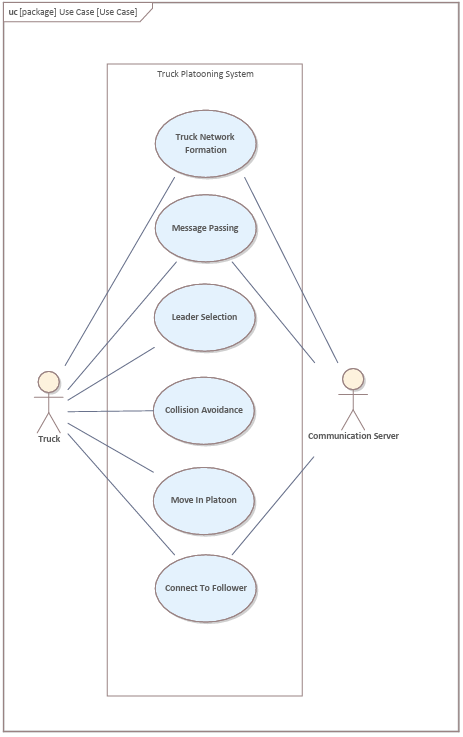
\includegraphics[width=0.4\textwidth]{images/usecase.png}
    \caption{System Use case}
    \label{img:usecase}
\end{figure}

\begin{itemize}
    \item Truck Network Formation 
    \item Message Passing
    \item Leader Selection 
    \item Collision Avoidance
    \item Move in Platoon 
    \item Connect To Follower
\end{itemize}
\textbf{Scenario for Implementation:} On analysis we come up with a scenario that potentially covers all the defined use cases. We consider a situation where a platoon of trucks with a leader and followers already exists and is connected over a communication server. In case of an error in the leader truck, we want to make sure that we can assign the role of leader to the truck that is in the first position of the platoon.
In the following section, we will discuss the design and implementation of the system.
 
